\documentclass[12pt]{report}

\usepackage{commands}


\begin{document}

\large

\begin{center}
 Math 586 Homework 4\\
 Due soon\\
 By Marvyn Bailly (GitHub: MarvynB)\\
\end{center}

\normalsize

\hrule

%---------------%
%---Problem 1---%
%---------------%

%--status--$

\begin{problem}
    Consider the implicit upwind method for the advection equation $u_t + a u_x = 0$
  \begin{align*}
    U_{j}^{n+1} = U_{j}^n  - \frac{ak}{h} \left( U_j^{n+1} - U_{j-1}^{n+1} \right).
  \end{align*}
  Derive the modified equation for this method to order $O(k + h)$.  Compare the effective diffusion coefficient with that of the modified equation for
  \begin{align*}
    U_{j}^{n+1} = U_{j}^n  - \frac{ak}{h} \left( U_j^{n} - U_{j-1}^{n} \right),
  \end{align*}
  which was derived in lecture.
\end{problem}

\begin{solution}

  \noindent
  Consider the implicit upwind method for the advection equation $u_t + a u_x = 0$
  \[
    U_{j}^{n+1} = U_{j}^n  - \frac{ak}{h} \left( U_j^{n+1} - U_{j-1}^{n+1} \right).
  \]
  Let's assume that $U^j_n = v(x_j,t_n)$ for a smooth function $v(x,t)$ and plugging this into the method yields
  \[ 
    \frac{v(x,t+k) - v(x,t)}{k} = -a \frac{v(x,t+k) - v(x-h,t+k)}{h}.
  \]
  Expanding the RHS yields
  \[
    \frac{v(x,t+k) - v(x,t)}{k} = v_t + \frac{k}{2}v_{tt} + \O(k^2),
  \]
  and expanding the LHS
  \begin{align*}
      \frac{v(x,t+k) - v(x-h,t+k)}{h} &= v_x(x,t+k) - \frac{h}{2}v_{xx}(x,t+k) + \O(h^2)\\
      &= \paren{v_x + kv_{xt} + \O(k^2)} - \frac{h}{2}\paren{v_{xx} +\O(k)}+ \O(h^2)\\
      &=v_x + kv_{xt} - \frac{h}{2}v_{xx} + \O(k^2 + kh + h^2).
  \end{align*}
  This gives
  \[
    v_t = -av_x - akx_{xt} + \frac{ah}{2}v_{xx} - \frac{k}{2}v_{tt}+ \O(k^2 + kh + h^2) = - av_x + \O (k +h).
  \] 
  Noticing that $v_t = -av_x + \O(k + h)$, we substitute $v_{xt} = - av_{xx} + \O(k + h)$ and $v_{tt} = a^2v_{xx} + \O(k + h)$ yielding
  \begin{align*}
    v_t &= av_x + \paren{a^2k + \frac{ah}{2} - \frac{ka^2}{2}}v_{tt}+ \O(k^2 + kh + h^2)\\
    &= av_x + \paren{\frac{ah}{2} + \frac{ka^2}{2}}v_{tt}+ \O(k^2 + kh + h^2).\\  
  \end{align*}
  Thus the diffusion constant is
  \[
    \frac{ah}{2} + \frac{ka^2}{2},
  \]
  and the PDE is well-posed if it is non-negative giving the condition
  \[
    \frac{ah}{2} + \frac{ka^2}{2} > 0 \implies \frac{ak}{h} \geq -1,
  \]
  for $a>0$. 
  
  \noindent
  On the other hand, recall that the modified equation for
  \[
    U_{j}^{n+1} = U_{j}^n  - \frac{ak}{h} \left( U_j^{n} - U_{j-1}^{n} \right),
  \]
  is given by
  \[
    v_{t} = -av_x + \paren{\frac{ah}{2} - \frac{a^2k}{2}}v_{xx} + \O(h^2 + hk + k^2),
  \]
  where the diffusion constant is
  \[
    \frac{ah}{2} - \frac{a^2k}{2}.
  \]
  This PDE is well-posed if the diffusion constant is non-negative
  \[
    \frac{ah}{2} - \frac{a^2k}{2} \geq 0 \implies \frac{ah}{k} \geq 1.
  \]


\end{solution}

%----------------------------------------------------------------------------------------------------%
%\vskip 20pt
\newpage

%---------------%
%---Problem 2---%
%---------------%

%--status--$

\begin{problem}
    Consider the method of lines discretization of the advection equation with a Dirichlet boundary conditions:
  $$ \begin{cases} u_t + a u_{x} = 0, \quad a > 0,\\
u(x,0) = \eta(x),\\
u(0,t) = g_0(t), \end{cases} $$
given by
\begin{align*}
  U'(t) &= A U(t) + g(t),\\
  A &= \frac{-a}{2h} \begin{bmatrix} 0 & 1 \\
    -1 & 0 & 1 \\
    & -1 & \ddots & \ddots \\
    && \ddots && 1\\
    &&& -1 & 0 \\
    &&1 & -4 & 3
  \end{bmatrix}, \quad g(t) = \begin{bmatrix} \frac{ak}{2h} g_0(t) \\ 0 \\ \vdots \\ 0 \end{bmatrix}.
\end{align*}
We have seen that if this is discretized using the leapfrog method then an instability is excited.  One may want to stabilize this in the way we stabilized forward Euler to obtain the Lax-Friedrichs method.  So, consider
\begin{align*}
  U_j^{n+1} = \frac 1 2 ( U_{j-1}^{n-1} + U_{j+1}^{n-1}) - \frac{ak}{h} ( U_{j+1}^n - U_{j-1}^n).
\end{align*}
Perform the von Neumann stability analysis to find $s(\xi)$ (LeVeque calls this $g(\xi)$) and give numerical evidence (or a proof, if you can) that $|s(\xi)| > 1$ for some $\xi$ regardless of $k,h$.  From this, one might conclude that $k \approx c h^2$ is required for stability.  Now, derive the modified equation and assess whether or not this restriction on $k$ is acceptable.
\end{problem}

\begin{solution}

    \noindent
    Consider the method of lines discretization of the advection equation with a Dirichlet boundary conditions:
  $$ \begin{cases} u_t + a u_{x} = 0, \quad a > 0,\\
u(x,0) = \eta(x),\\
u(0,t) = g_0(t), \end{cases} $$
given by
\begin{align*}
  U'(t) &= A U(t) + g(t),\\
  A &= \frac{-a}{2h} \begin{bmatrix} 0 & 1 \\
    -1 & 0 & 1 \\
    & -1 & \ddots & \ddots \\
    && \ddots && 1\\
    &&& -1 & 0 \\
    &&1 & -4 & 3
  \end{bmatrix}, \quad g(t) = \begin{bmatrix} \frac{ak}{2h} g_0(t) \\ 0 \\ \vdots \\ 0 \end{bmatrix}.
\end{align*}
We have seen that if this is discretized using the leapfrog method then an instability is excited.  One may want to stabilize this in the way we stabilized forward Euler to obtain the Lax-Friedrichs method.  So, consider
\begin{align*}
  U_j^{n+1} = \frac 1 2 ( U_{j-1}^{n-1} + U_{j+1}^{n-1}) - \frac{ak}{h} ( U_{j+1}^n - U_{j-1}^n).
\end{align*}
To preform von Neumann stability analysis, let $U_j^n = s(\xi)^h e^{ij\xi h}$ and substituting this into our equation we have
\[ 
  s(\xi)^{n+1}e^{ij\xi h} = \frac{1}{2}\paren{s(\xi)^{n-1}e^{i(j-1)\xi h} + s(\xi)^{n-1}e^{i(j-1)\xi h}} - \frac{ak}{h}\paren{s(\xi)^n e^{i(j+1)} + s(\xi)^n e^{i(j-1)}},
\] 
and dividing through by $s(\xi)^{n-1}e^{ij\xi h}$ yields
\[
  s(\xi)^2  = \frac{1}{2}\paren{e^{-i\xi h} + e^{i \xi h}} - \frac{ak}{h}s(\xi)\paren{e^{i\xi h} - e^{-i\xi h}} = \cos(\xi h) - \frac{ak}{h}s(\xi)2i\sin(\xi h).
\]
Now solving for $s(\xi)$ we get 
\[
  s(\xi)^2 + \nu 2i\sin(\xi h)s(\xi) - \cos(\xi h) = 0,
\]
where $\nu = \frac{ak}{h}$ and thus we find that 
\[
  s(\xi) = - i \nu \sin(\xi h) \pm \sqrt{\cos(\xi h) - \nu \sin^2(\xi h)}.
\]
Now we wish to show that $|s(\xi)| > 1$ for some $\xi$ regardless of $k,h$. Consider when $\xi_1 = \pi/h$, then 
\[
  s(\xi_1) = 0 \pm \sqrt{\cos(\pi) - 0} = \pm i,
\]
and thus 
\[
  |s(\xi_1)| = 1.
\]
Now if we compute the derivative we get
\[ 
  s'(\xi) = -ih\nu \cos(\xi h) \mp \frac{h \sin(\xi h)(2\nu^2\cos(\xi h) + 1)}{2\sqrt{-\nu^2 \sin^2{\xi h} + \cos(\xi h)}}.
\]
Notice that $s'(\xi_1) = ih\nu$ and since $s(\xi)$ is known to be continuous, there must exist some $\xi$ such that the real part is zero and $|s(\xi)| > 1$. Therefore we might conclude that $k\approx ch^2$ may be required for stability. To access if this restriction on $k$ is acceptable, we derive the modified equation. Consider $U^j_n = v(x,t)$ for a sufficiently smooth function $v(x,t)$. Plugging this in yields
\[
 v(x,t+k) = \frac{1}{2}\paren{v(x-h,t-k) + v(x+h,t-k)}  - \frac{ak}{h}\paren{v(x+h,t) - v(x-h,t)}.
\]
Now Taylor expanding the left-hand side gives
\[
  v(x,t+k) = v + kv_t + \frac{k^2}{2}v_{tt} + \O(k^3),
\]
and Taylor expanding the first term on the right-hand side gives
\begin{align*}
  \frac{1}{2}\paren{v(x-h,t-k) + v(x+h,t-k)} &= \frac{1}{2}\paren{2v(x,t-k) + h^2v_{xx} + \O(h^4)}\\
  &= v(x,t-k) + \frac{h^2}{2}v_{xx}(x,t-k) + \O(h^4)\\
  &= \paren{v - kv_t + \frac{k^2}{2}v_{tt} + \O(k^3)} + \frac{h^2}{2}\paren{v_{xx} + \O(k)} + \O(h^4)\\
  &= v - kv_t + \frac{k^2}{2}v_{tt} + \frac{h^2}{2}v_{xx} + \O(k^4+ h^2k + k^3).
\end{align*}
Taylor expanding the second term on the right-hand side gives
\begin{align*}
  \frac{ak}{h}\paren{v(x+h,t) - v(x-h,t)} &= \frac{ak}{h}\paren{2hv_x + \O(h^3)}\\
  &= 2akv_x + \O(kh^2).
\end{align*}
Thus the equation becomes 
\[
  v + kv_t + \frac{k^2}{2}v_{tt} + \O(k^3) = v - kv_t + \frac{k^2}{2}v_{tt} + \frac{h^2}{2}v_{xx} + \O(k^4+ h^2k + k^3) + 2akv_x + \O(kh^2),
\]
which we can solve for $v_t$ to get the modified equation to be
\[
  v_t = - av_x + \frac{h^2}{4k}v_{xx} + \O(\frac{h^4}{k} + h^2 + k^2).  
\]
Then if we let $k \approx ch^2$ the equation becomes
\[
  v_t \approx = -av_x + \frac{1}{4c}v_{xx} + \O(h^2).
\]
Notice that while the diffusion coefficient is nonnegative, the method is not consistent as $\frac{1}{4c}v_{xx} \not\to 0$ as $k,h \to \infty$ and therefore will not converge. Thus we can conclude that this restriction on $k$ is not acceptable. 

\end{solution}

%----------------------------------------------------------------------------------------------------%
%\vskip 20pt
\newpage

%---------------%
%---Problem 3---%
%---------------%

%--status--$

\begin{problem}
    Consider the wave equation with periodic boundary conditions on $[0,1]$
  \begin{align*}
    \begin{cases}
      u_{tt} = c^2 u_{xx}, \quad c > 0,\\
      u(x,0) = f(x),\\
      u_t(x,0) = g(x),\\
      u(0,t) = u(1,t),\\
      u_x(0,t) = u_x(1,t).
    \end{cases}
  \end{align*}
  Using $f(x) = \exp( -20(x-1/2)^2 )$, $g(x) = \sin(4\pi x)$, $c = 1$, implement a method to compute and plot the solution at $t = 0,1,2,3$ with $h = 0.01$.  The $k$ you need to choose will depend on the method you use.  Describe your method in detail. 
\end{problem}

\begin{solution}

    \noindent
    Consider the wave equation with periodic boundary conditions on $[0,1]$\begin{align*}
      \begin{cases}
        u_{tt} = c^2 u_{xx}, \quad c > 0,\\
        u(x,0) = f(x),\\
        u_t(x,0) = g(x),\\
        u(0,t) = u(1,t),\\
        u_x(0,t) = u_x(1,t),
      \end{cases}
    \end{align*}
    where $f(x) = \exp( -20(x-1/2)^2 )$, $g(x) = \sin(4\pi x)$, $c = 1$. Observe that
    \[
      u_{tt} - c^2 u_{xx} = \paren{\partial_t - c \partial_x}\paren{\partial_t + c \partial_x}u = 0,
    \]
    and thus if we let $v = (v_1(x,t),v_2(x,t))$ where $v_1(x,t) = u(x,t)$ and $v_2(x,t) = \paren{\partial_t + c \partial_x}u$ then
    \[ 
      v_t + c \begin{bmatrix}
        1 & 0\\ 0 & -1
      \end{bmatrix}v_x = \begin{bmatrix}
        0 & 1 \\ 0 & 0
      \end{bmatrix}v.
    \]
    Then the boundary conditions become
    \begin{align*}
      v_1(0,t) &= u(0,t) = u(1,t) = v_1(1,t),\\
      v_2(0,t) &= u_t(0,t) + cu_x(0,t) = u_t(1,t) + cu_x(1,t) = v_2(1,t), 
    \end{align*}
    and the initial conditions are
    \begin{align*}
      v_1(x,0) &= u(x,0) = f(x),\\
      v_2(x,0) &= u_t(x,0) + c u_x(x,0) = g(x) + c f'(x).
    \end{align*}
    Now we are trying to solve the two equations
    \[
      \begin{cases}
        v_{2,t} - c v_{2,x} = 0\\
        v_{1,t} + c v_{1,x} = v_2.
      \end{cases}
    \]
    Noting that the first equation is completely independent of $v_1$, we can solve it using the Lax-Wendroff method to get
    \[
      [V_{2,j}^{n+1}] = \paren{I + \frac{ck}{2h}S - \frac{c^2k^2}{2h^2}A}[V_{2,j}^n],
    \]
    where
    \[
      S = \begin{bmatrix}
        0 & 1 & & & -1 \\
        -1 & 0 & 1 \\
        & \ddots & \ddots & \ddots\\
        && -1 & 0 & 1 \\
        1&&& -1 & 0
    \end{bmatrix},
    \]
    and
    \[
      A = \begin{bmatrix}
        2 & -1 & & & -1 \\
        -1 & 2 & -1 \\
        & \ddots & \ddots & \ddots\\
        && -1 & 2 & -1 \\
        -1&&& -1 & 2
    \end{bmatrix}.
    \]
    Since this method will give us the $V_{2,j}^n$ for any $j$, we can use Lax Wendroff to get
    \[
      [V_{1,j}^{n+1}] = \paren{I - \frac{ck}{2h}S - \frac{c^2k^2}{2h^2}A}[V_{1,j}^n] + k[V_{2,j}^n].
    \]
    For stability, we require that
    \[ 
      \left| \frac{ck}{h} \right| = \frac{ck}{h} \leq 1
    \]
    and thus we let $h = 0.01$ and $k = h$. This method is implemented in Julia using the following code:
    \begin{python}
    f = x -> exp(-20*(x - 1/2)^2)
    df = x -> -40*(x - 1/2)*exp(-20*(x - 1/2)^2)
    g = x -> sin(4 * pi * x)

    function solve_wave(m,c,stop)
        h = 1/(1+m)
        k = h
        xs = h:h:1-h

        S = Tridiagonal(fill(-1.0,m-1),fill(0.0,m),fill(1.0,m-1)) |> sparse
        S[1,end] = -1
        S[end,1] = 1

        A = SymTridiagonal(fill(2.0,m),fill(-1.0,m-1)) |> sparse
        A[1,end] = -1
        A[end,1] = -1

        v1 = map(f, xs)
        v2 = map(g, xs) + c*map(df,xs)

        for t=0:k:stop 
            v2 = (I + (c*k)/(2*h) * S - (c^2*k^2)/(2*h^2) * A)*v2;
            v1 = (I - (c*k)/(2*h) * S - (c^2*k^2)/(2*h^2) * A)*v1 + k*v2
        end
        return xs, v1
    end
    \end{python}
    Using the described method, we plot the solution for $t = 0,1,2,3$ which can be seen in Figure 1. While the solution between times looks similar, we see the begins of an unstablity growing with time.

    \begin{figure}[H] \label{fig:3}
      \centering
      \begin{subfigure}{0.495\linewidth}
        \centering
        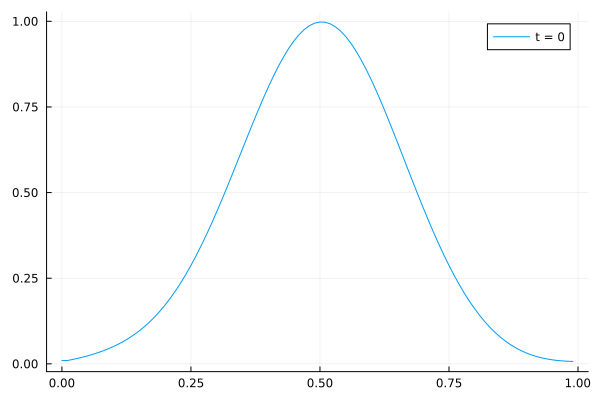
\includegraphics[width=\linewidth]{images/3-1.png}
      \end{subfigure}
      \begin{subfigure}{0.495\linewidth}
        \centering
        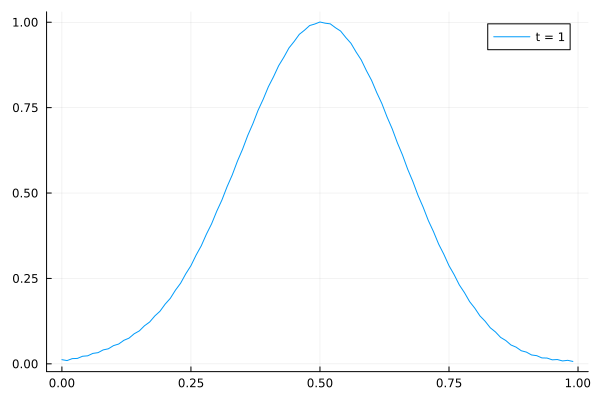
\includegraphics[width=\linewidth]{images/3-2.png}
      \end{subfigure}
      \begin{subfigure}{0.495\linewidth}
        \centering
        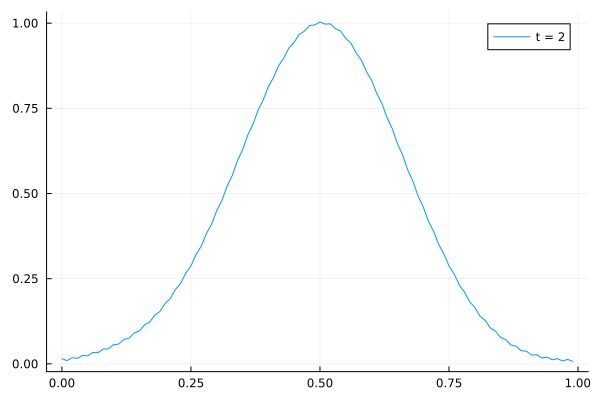
\includegraphics[width=\linewidth]{images/3-3.png}
      \end{subfigure}
      \begin{subfigure}{0.495\linewidth}
        \centering
        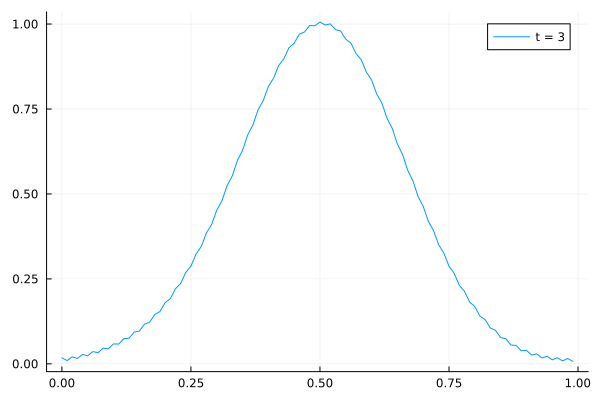
\includegraphics[width=\linewidth]{images/3-4.png}
      \end{subfigure}
      \caption{Solutions for $t\in[0,1,2,3]$.}
    \end{figure}
\end{solution}

%----------------------------------------------------------------------------------------------------%
%\vskip 20pt
\newpage

%---------------%
%---Problem 4---%
%---------------%

%--status--$

\begin{problem}
    Consider the non-constant coefficient reaction diffusion equation
  \begin{align*}
    \begin{cases}
      u_t = \kappa(x) u_{xx} + u(1-u)(u-1/2), \quad \kappa(x) = \sin^4(2\pi x - \pi),\\
      u(x,0) = \eta(x),\\
      u(0,t) = u(1,t),\\
      u_x(0,t) = u_x(1,t).
    \end{cases}
  \end{align*}
  Use the initial condition
  \begin{align*}
    \eta(x) = \frac{ ( 1 + \mathrm{tanh}(20(x-0.25)) ) ( 1 + \mathrm{tanh}(20(-x+0.75)))}{4}.
  \end{align*}
  Solve this problem by forming the diffusion matrix
  \begin{align*}
    A_{\kappa} = \frac{1}{h^2} \mathrm{diag}(\kappa(x_1),\ldots,\kappa(x_m)) A, \quad A  = \begin{bmatrix}
-2  & 1 &&& 1\\
1 & -2 & 1 \\
& 1 & -2 & 1\\
&& \ddots & \ddots & \ddots \\
1&&& 1 & -2 \end{bmatrix}.
  \end{align*}
  Write a function {\tt CN(U,k)} that performs a step of size $k$ for trapezoid applied to the MOL discretization $U'(t) = A_{\kappa} U(t)$.  Next use RK2 (5.30) to write a function {\tt RK2(U,k)} performs one time step of $U'(t) = U(t)(1-U(t))(U(t) - 1/2)$ with time step $k$.  Note that while we are solving a PDE, the MOL discretization of a term without derivatives is a system of uncoupled ODEs.  The Strang splitting scheme for this problem is then written as:
\begin{verbatim}
  U = RK2(U,k/2)
  U = CN(U,k)
  U = RK2(U,k/2)
\end{verbatim}
Use this scheme to plot the solution at $t = 0.01,0.10,1.00$.  Repeat with $\kappa(x) = \cos^4(2\pi x)$.
\end{problem}

\begin{solution}

    \noindent
    Consider the non-constant coefficient reaction-diffusion equation
    \begin{align*}
      \begin{cases}
        u_t = \kappa(x) u_{xx} + u(1-u)(u-1/2),\\
        u(x,0) = \eta(x),\\
        u(0,t) = u(1,t),\\
        u_x(0,t) = u_x(1,t),
      \end{cases}
    \end{align*}
    where $\kappa(x) = \sin^4(2\pi x - \pi)$ and
    \begin{align*}
      \eta(x) = \frac{ ( 1 + \mathrm{tanh}(20(x-0.25)) ) ( 1 + \mathrm{tanh}(20(-x+0.75)))}{4}.
    \end{align*}
    To solve this equation, we will use the diffusion matrix 
    \begin{align*}
      A_{\kappa} = \frac{1}{h^2} \mathrm{diag}(\kappa(x_1),\ldots,\kappa(x_m)) A, \quad A  = \begin{bmatrix}
  -2  & 1 &&& 1\\
  1 & -2 & 1 \\
  & 1 & -2 & 1\\
  && \ddots & \ddots & \ddots \\
  1&&& 1 & -2 \end{bmatrix},
    \end{align*}
    with the Crank-Nicolson method along with the RK2 method. We created the Crank-Nicolson method using the following Julia code:
    \begin{python}
    function CN(U,k)
      h = k
      m = convert(Int64,1/h)-1
      xs = h:h:1-h
      A = SymTridiagonal(fill(-2.0,m),fill(1.0,m-1)) |> sparse
      A[1,end] = 1
      A[end,1] = 1
      diag = Diagonal(map(k,xs)) |> Matrix
      Ak = (1/h^2) * diag * A
      U = (I - (k/2) * Ak) \ (I + (k/2) * Ak)*U    
    end
    \end{python}
    We created the RK2 method that performs $U'(t) = U(t)(1-U(t))(U(t) - 1/2)$ with time step $k$ with the following Julia code:
    \begin{python}
    function RK2(U,k)
      f = u -> u*(1 - u)*(u - 1/2)
      U1 = U + k/2*(map(f,U))
      U2 = U1 + k*map(f,U)
    end
    \end{python}
    Then we used the Strange splitting scheme:
    \begin{verbatim}
      U = RK2(U,k/2)
      U = CN(U,k)
      U = RK2(U,k/2)
    \end{verbatim}
    to solve the problem at $t\in[0.01,0.10,1.00]$ which can be seen in Figure 2. We repeated the process but with $\kappa(x) = \cos^4(2\pi x)$ to get the results seen in Figure 3. 
    \begin{figure}[H] \label{4a}
      \centering
      \begin{subfigure}{0.495\linewidth}
        \centering
        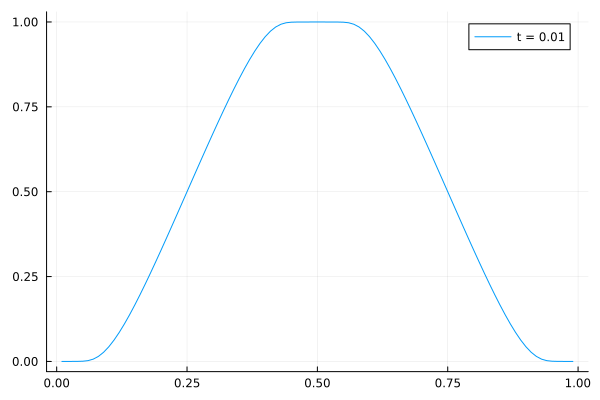
\includegraphics[width=\linewidth]{images/4a-1.png}
      \end{subfigure}
      \begin{subfigure}{0.495\linewidth}
        \centering
        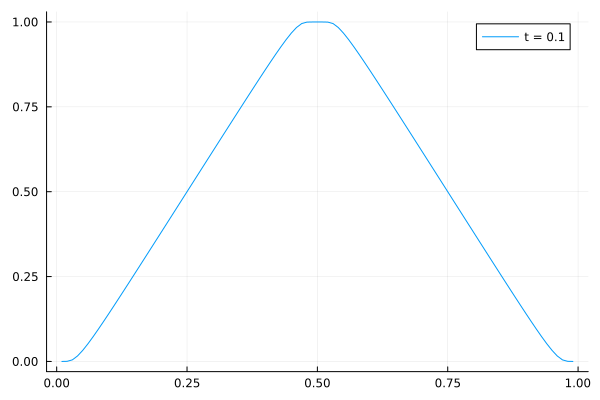
\includegraphics[width=\linewidth]{images/4a-2.png}
      \end{subfigure}
      \begin{subfigure}{0.495\linewidth}
        \centering
        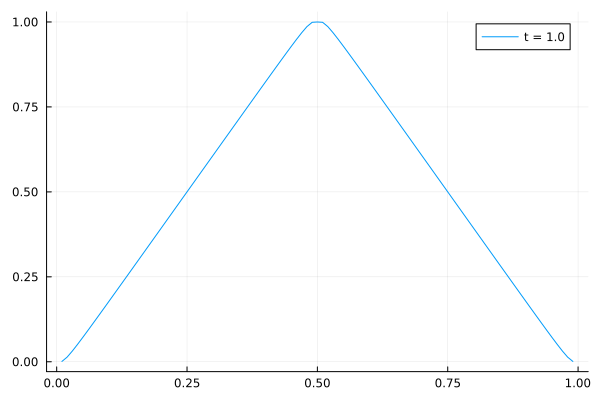
\includegraphics[width=\linewidth]{images/4a-3.png}
      \end{subfigure}
      \caption{Solutions for $t\in[0.01,0.10,1.00]$ using the Strange splitting scheme with $\kappa(x) = \sin^4(2\pi x - \pi)$.}
    \end{figure}
    \begin{figure}[H]\label{4b}
      \centering
      \begin{subfigure}{0.495\linewidth}
        \centering
        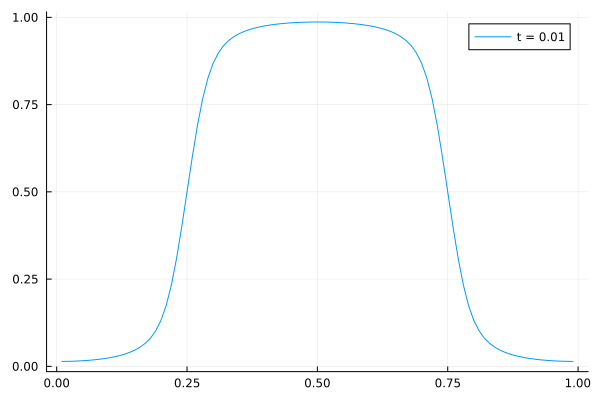
\includegraphics[width=\linewidth]{images/4b-1.png}
      \end{subfigure}
      \begin{subfigure}{0.495\linewidth}
        \centering
        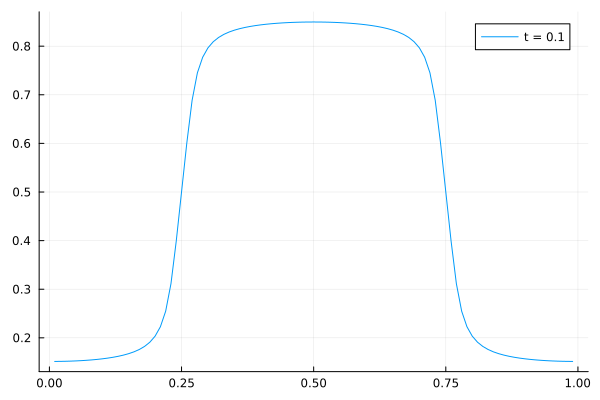
\includegraphics[width=\linewidth]{images/4b-2.png}
      \end{subfigure}
      \begin{subfigure}{0.495\linewidth}
        \centering
        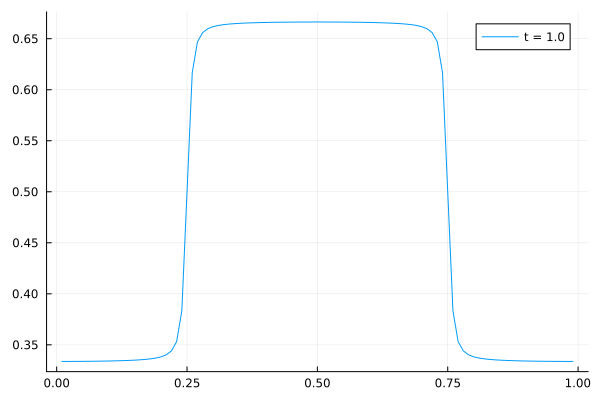
\includegraphics[width=\linewidth]{images/4b-3.png}
      \end{subfigure}
      \caption{Solutions for $t\in[0.01,0.10,1.00]$ using the Strange splitting scheme with $\kappa(x) = \cos^4(2\pi x)$.}
    \end{figure}


  \end{solution}

%----------------------------------------------------------------------------------------------------%
%\vskip 20pt
\newpage

%---------------%
%---Problem 5---%
%---------------%

%--status--$

\begin{problem}
    Prove that for two $n \times n$ matrices $A$, $B$ that
  \begin{align*}
    e^{k(A+B)} - e^{k/2 A}e^{k B}e^{k/2 A} = O(k^3).
  \end{align*}
\end{problem}

\begin{solution}

    \noindent
    Consider the two $n \times n$ matrices $A$ and $B$. Observe that Taylor expanding matrix exponential yields
    \begin{align*}
        e^{k(A+B)} &= I + k(A+B) + \frac{k^2}{2}(A+B)^2 + \O(k^3)\\
        &= I + k(A+B) + \frac{k^2}{2}(A^2+AB+BA+B^2) + \O(k^3)
    \end{align*}
    and
    \begin{align*}
        e^{k/2A}  e^{k B} e^{k/2 A} &= \paren{I + \frac{kA}{2} + \frac{k^2A^2}{8} + \O(k^3)}\paren{I + kB + \frac{k^2B^2}{2} + \O(k^3)}\paren{I + \frac{kA}{2} + \frac{k^2A^2}{8} + \O(k^3)}\\
        &=\paren{I + k\paren{\frac{A}{2} + B} + k^2\paren{\frac{A^2}{8} + \frac{AB}{2} + \frac{B^2}{2}} + \O (k^3)}\paren{I + \frac{kA}{2} + \frac{k^2A^2}{8} + \O(k^3)}\\
        &=I + k\paren{A + B} + k^2\paren{\frac{A^2}{8} + \frac{AB}{2} + \frac{B^2}{2} + \frac{A^2}{8} + \frac{A^2}{4} + \frac{BA}{2}} +\O (k^3)\\
        &=I + k\paren{A + B} + k^2\paren{\frac{A^2}{2} + \frac{BA}{2} + \frac{B^2}{2} + \frac{AB}{2}} +\O (k^3)\\
        &=I + k\paren{A + B} + \frac{k^2}{2}\paren{A^2 + AB + BA + B^2} +\O (k^3).\\
    \end{align*}
    Thus we have that
    \[ 
        e^{k(A+B)} - e^{k/2A}  e^{k B} e^{k/2 A} = \O(k^3).
    \]

\end{solution}

%----------------------------------------------------------------------------------------------------%
%\vskip 20pt
\newpage

%---------------%
%---Problem 6---%
%---------------%

%--status--$

\begin{problem}
    Consider the Jacobi iteration (4.4) for the linear system $A u=f$ arising from a centered difference approximation of the boundary value problem $u_{x x}(x)=f(x)$. Show that this iteration can be interpreted as forward Euler time stepping applied to the MOL equations arising from a centered difference discretization of the heat equation $u_{t}(x, t)=u_{x x}(x, t)-f(x)$ with time step $k=\frac{1}{2} h^{2}$.
  
  Note that if the boundary conditions are held constant then the solution to this heat equation decays to the steady state solution that solves the boundary value problem. Marching to steady state with an explicit method is one way to solve the boundary value problem, though as we saw in Chapter 4 this is a very inefficient way to compute the steady state. 
\end{problem}

\begin{solution}

    \noindent
    Consider the boundary value problem $u_{xx} = f(x)$. Using a centered difference approximation we can rewrite the problem as $Au = f$. Applying Jacobi iteration to the linear system yields
    \begin{equation} \label{6sol}
      u_{j}^{n+1} = \frac{1}{2}\paren{u_{j-1}^{n} + u_{j+1}^{n} - h^2 f_i}.      
    \end{equation}
    We wish to show that the iteration in \fullref{6sol} is analogous to a forward Euler applied to the MOL using a centered difference discretization of the heat equation
    \[
      u_t = u_{xx} - f.
    \]
    Applying the MOL to the heat equations yields
    \[
      U'_j(t) = \frac{U_{j+1}(t) - 2U_j(t) + U_{j-1}(t)}{h^2} - f_j.
    \]
    Next, we apply forward Euler
    \[
      \frac{U_{j}^{n+1}(t) - U_{j}^{n}(t)}{k} = \frac{U_{j+1}(t) - 2U_j(t) + U_{j-1}(t)}{h^2} - f_j,
    \]
    and letting the step size be $k = \frac{1}{2}h^2$ gives
    \begin{align*}
      \frac{U_{j}^{n+1}(t) - U_{j}^{n}(t)}{h^2/2} &= \frac{U_{j+1}^n(t) - 2U_j^n(t) + U_{j-1}^n(t)}{h^2} - f_j,\\
      U_{j}^{n+1}(t) - U_{j}^{n}(t) &= \frac{1}{2}\paren{U_{j+1}^n(t) - 2U_j^n(t) + U_{j-1}^n(t)} - \frac{h^2}{2}f_j\\
      U_{j}^{n+1}(t) &= \frac{1}{2}\paren{U_{j+1}^n(t) + U_{j-1}^n(t) - h^2f_j},\\
    \end{align*}
    which is analogous to \fullref{6sol}. Thus we have shown Jacobi iteration applied to the linear system Au = f arising from a centered difference approximation of the boundary value problem $u_{xx} = f$ can be interpreted as forward Euler time stepping applied to the MOL equations arising from a centered difference discretization of the heat equation $u_t = u_{xx} - f$ with time step $k = \frac{1}{2}h^2$. 

\end{solution}

%----------------------------------------------------------------------------------------------------%
%\vskip 20pt
\newpage

%---------------%
%---Problem 7---%
%---------------%

%--status--$

\begin{problem}
    From the previous problem, we see that the Jacobi iteration for solving the boundary value problem $u_{x x}(x)=f(x)$ can be viewed as an explicit time-stepping method for the heat equation $u_{t}(x, t)=u_{x x}(x, t)-f(x)$ with a time step $k=h^{2} / 2$. Now consider the Gauss-Seidel method for solving the linear system,
    $$
      U_{j}^{n+1}=\frac{1}{2}\left(U_{j-1}^{n+1}+U_{j+1}^{n}-h^{2} f\left(x_{j}\right)\right)
    $$
    This can be viewed as a time stepping method for some PDE. Compute the modified equation for this finite difference method and determine what PDE it is consistent with if we let $k=h^{2} / 2$ again. Comment on how this relates to the observation in Section 4.2.1 that Gauss-Seidel takes roughly half as many iterations as Jacobi to converge.
\end{problem}

\begin{solution}

  \noindent
  Consider the Gauss-Seidel method for solving the linear system
  \[
    U_j^{n+1} = \frac{1}{2}\paren{U^{n+1}_{j-1} + U^n_{j+1}- h^2f(x_j)}.
  \]
  To figure out which PDE this time stepping method solves, we will compute the modified equation by assuming $U_j^n = v(x_j,t_n)$ for a smooth function $v(x,t)$ and plugging this into the method yields
  \[ 
    2v(x,t+k) = v(x-h,t+k) + v(x+h,t) - h^2f(x).
  \]
  Now Taylor expanding the left-hand side gives
  \[
    2v + 2kv_t + k^2 v_{tt} + \O(k^3),
  \]
  and Taylor expanding the right-hand sides gives
  \begin{align*}
    v(x-h,t+k) + v(x+h,t) - h^2f(x) &= \paren{ v(x,t+k) - hv_x(x,t+k) + \frac{h^2}{2}v_{xx}(x,t+k)}\\
    &\quad + \paren{v(x,t) + hv_x(x,t) + \frac{h^2}{2}v_{xx}(x,t)} - h^2f + \O(h^3)\\
    &= \paren{v + kv_t + k^2v_{tt} + \O(k^3)} - h\paren{v_x + kv_{xt} + \O(k^2)}\\
    &\quad + \frac{h^2}{2}\paren{v_{xx} + \O(k)} + v + hv_x + \frac{h^2}{2}v_{xx} - h^2f(x) + \O(h^3)\\
    &= 2v + kv_t + h^2v_{xx} + k^2v_{tt} - khv_{xt} - h^2f(x) \\
    &\quad + \O(h^3 + k^2h + h^2k + k^3).
  \end{align*}
  Thus we have the modified equation to be
  \[
    v_t = \frac{h^2}{k}v_{xx} - hv_{xt} - \frac{h^2}{k}f(x) + \O(h^3 + kh + h^2k + k^2),
  \]
  and letting $k=h^2/2$ gives
  \[
    v_t = 2v_{xx} - hv_{xt} - 2f(x) + \O(h^2) = 2(v_{xx} - f(x)) + \O(h).
  \]
  Thus we see that if we let time step with $k = h^2/2$, then the Gauss-Seidel method for solving the linear system
  \[
    U_j^{n+1} = \frac{1}{2}\paren{U^{n+1}_{j-1} + U^n_{j+1}- h^2f(x_j)}.
  \]
  is consistent with the PDE
  \[
    u_t = 2(u_{xx}(x,t) - f(x)).
  \]
  In Problem 6, we found that Jacobi iteration for the linear system $Au = f$ arising from a centered difference approximation of the boundary value problem $u_{xx}(x) = f(x)$ can be interpreted as solving $u_t(x,t) = u_{xx}(x,t) - f(x)$. Notice that this is $1/2$ the RHS as the solution we PDE we found above and thus it makes sense that Gauss-Seidel takes roughly half the time as many iterations as Jacobi to converge.



\end{solution}

%----------------------------------------------------------------------------------------------------%
%\vskip 20pt
\newpage


\end{document}